\chapter{Results}
This chapter shows the results of the experiment and how the gathered data can be interpreted. 

The results.......................................................................
\bigbreak

\iffalse %Something like uncommenting (START)

\begin{adjustbox}{width=\textwidth}
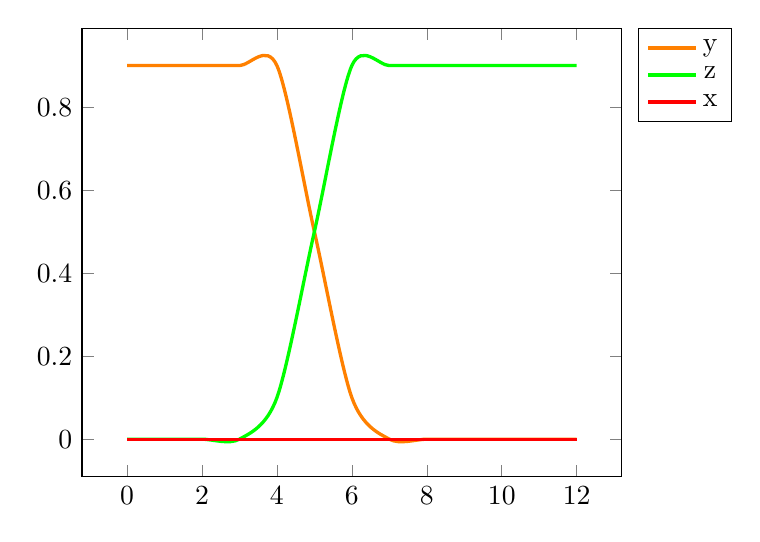
\begin{tikzpicture}
\begin{axis}[domain=0:1,legend pos=outer north east]
\addplot[orange,very thick][smooth]coordinates {(0,0.9)(1,0.9)(2,0.9)(3,0.9)(4,0.9)(5,0.5)(6,0.1)(7,0)(8,0)(9,0)(10,0)(11,0)(12,0)};
\addplot[green,very thick][smooth]coordinates {(0,0)(1,0)(2,0)(3,0)(4,0.1)(5,0.5)(6,0.9)(7,0.9)(8,0.9)(9,0.9)(10,0.9)(11,0.9)(12,0.9)};
\addplot[red,very thick]coordinates {(0,0)(12,0)};

\legend{y,z,x}

\end{axis}
\end{tikzpicture}
\end{adjustbox}


\begin{figure}
	\centering
	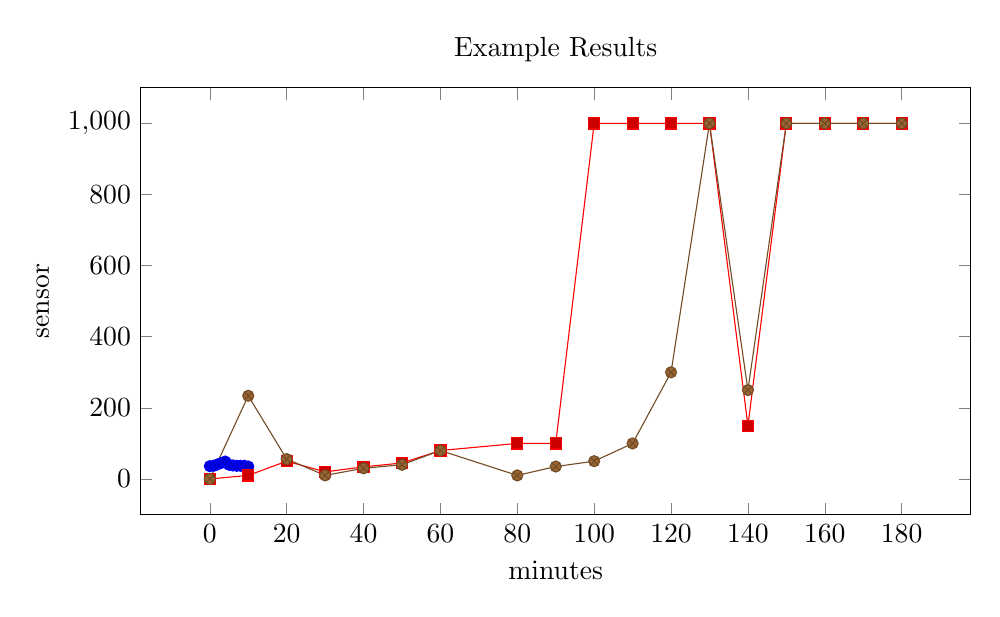
\begin{tikzpicture}
\begin{axis}[
	height=7cm,
	width=\textwidth,
	xlabel=minutes,
	ylabel=sensor,
	title=Example Results,
	unbounded coords=discard],
	
	
	\addplot coordinates {
		(0,36.0)
		(1,37.0)
		(2,41.0)
		(3,45.0)
		(4,49.0)
		(5,40.0)
		(6,38.0)
		(7,37.0)
		(8,37.0)
		(9,37.0)
		(10,35.0)
	};
	
			
\addplot coordinates {
		(0,0) 
		(10,10) 
		(20,50) 
		(30,20) 
		(40,34) 
		(50,45) 
		(60,80) 
		(80,100)
		(90,100)
		(100,1000)
		(110,1000)
		(120,1000)
		(130,1000)
		(140,150)
		(150,1000)
		(160,1000)
		(170,1000)
		(180,1000)
	};	
	
	\addplot coordinates {
		(0,0) 
		(10,234) 
		(20,56) 
		(30,10) 
		(40,30) 
		(50,40) 
		(60,80) 
		(80,10)
		(90,35)
		(100,50)
		(110,100)
		(120,300)
		(130,1000)
		(140,250)
		(150,1000)
		(160,1000)
		(170,1000)
		(180,1000)
	};	
	
	

	

\end{axis}
\end{tikzpicture}
 	\vspace{10 mm}
\end{figure}

\fi %Something like uncommenting (END)